% Leo's LaTeX guide to writing a Master's thesis
\documentclass[masters,en,listoffigures,listoftables,acronyms]{NMBU}

\usepackage{booktabs}
\usepackage{tabularx}
\usepackage{microtype}
\usepackage{siunitx}
\usepackage{soul}
\usepackage{float}
\usepackage[font=small,labelfont=bf]{caption}
\usepackage[most]{tcolorbox}

\usetikzlibrary{arrows.meta,positioning}

% A small visual vocabulary for examples. The labels carry the meaning, so the
% boxes remain understandable when printed in greyscale.
\definecolor{GuideGreen}{HTML}{DBF8F4}
\definecolor{GuideGreenDark}{HTML}{025C4F}
\definecolor{GuideRed}{HTML}{EFC3CD}
\definecolor{GuideRedDark}{HTML}{DB003A}
\definecolor{GuideBlue}{HTML}{D4DDEF}
\definecolor{GuideBlueDark}{HTML}{5967A6}
\definecolor{GuideGold}{HTML}{FFD757}
\definecolor{GuideGoldDark}{HTML}{0D3B34}

\tcbset{
  guidebox/.style={
    enhanced,
    breakable,
    boxrule=0.6pt,
    arc=1mm,
    left=2mm,
    right=2mm,
    top=1.5mm,
    bottom=1.5mm,
    fonttitle=\bfseries,
  },
  guideblue/.style={
    guidebox,
    colback=GuideBlue,
    colframe=GuideBlueDark,
  },
  guidered/.style={
    guidebox,
    colback=GuideRed,
    colframe=GuideRedDark,
  },
  guidegreen/.style={
    guidebox,
    colback=GuideGreen,
    colframe=GuideGreenDark,
  },
  guidegold/.style={
    guidebox,
    colback=GuideGold,
    colframe=GuideGoldDark,
  },
}

\newtcolorbox{thesispoint}[1]{
  guideblue,
  title={#1},
}

\newtcolorbox{avoidbox}[1]{
  guidered,
  title={#1},
}

\newtcolorbox{betterbox}[1]{
  guidegreen,
  title={#1},
}

\newtcolorbox{latexnote}[1]{
  guidegold,
  title={#1},
}

\newcolumntype{Y}{>{\raggedright\arraybackslash}X}

\addbibresource{bib.bib}

\title{How to Write a Master's Thesis Like a Champ, or Whatever}
\author{Leo's \LaTeX~guide to getting your thesis done}
\thesisyear{Guide}
\credits{}
\faculty{Faculty of Science and Technology}
\studyprogramme{Environmental Physics and Renewable Energy}
\supervisor{Ahhh, Leo here, how are you doing?}
% \engtitle{} % Required only when the thesis is written in a Scandinavian language.

% Front matter is declared here and printed automatically by the class.
\abstract{This document is an example thesis that deliberately contains no original research.
Its aim is to try to help get your Master's thesis from a bundle of words to a precise research question, and from theory, literature, methods, and results to a defensible conclusion. We will go throught a few examples of what works and what does not work.
Number one thing that does not work: your Python installation.
Number two thing that does not work: not having backups! That is definitely not work.
Keep a backup, always!
Anyway.
How do we write this thesis? Well, the principal finding is that clear writing usually follows clear thinking, coffee, careful revision, a second coffee, and regular conversations with a supervisor, mostly with coffee involved as well.
This template cannot perform those tasks, although it will number the pages very reliably.
Did I mention coffee?}

\acknowledgements{The author thanks the supervisor for asking, repeatedly and with admirable restraint, `What exactly do you mean by this sentence?' The coffee provided logistical support. A sponsorship by the oil directorate would have been welcome, mainly for beer money. The author only takes credit for the good results. The other results are just due to statistical variability, or whatever. Oh, and thank your parents or those that raised you, they are generally cool people.}

\begin{document}

\startthesis

\section{Introduction: The magic funnel}\label{sec:introduction}

Congratulations. You have reached the stage at which notes, scripts, plots, half-finished paragraphs, and files named \texttt{final-final-really-final-7} must become a Master's thesis.
This is possible.
They say it can be done.
They say it should be done.
At the same time, it has been a while since you wrote a 50-page document.
Now that you think of it, it has never happened before.
Hmm, that is\dots fine, totally fine, chill, no worries, tots relaxed.

So, what is all this fuss about theses\footnote{Yup, that is the plural of `thesis': `theses'. Shame really, `thesises' or `thesiseses' would have been nicer to say.}? A thesis is not an archaeological record of everything that happened during the project -- although some supervisors can be classified as fossils at some later stages of their academic careers.
A thesis is a reasoned answer to a defined research problem.
I guess that is\footnote{Some of your avid English writers might be wondering `why did we not use a contraction here and write \emph{that's}?'. That was not what you were thinking? Ouh, that is odd \dots Well, anyway, in thesis writing we \st{don't} do not use unnecessary contractions. Possessive terms are fine, such as `\emph{the author's argument}', but other contractions should be avoided.} why it is called a \emph{thesis}, i.e.,\footnote{If you want to sound super academic, use things like `i.e.' (that is) and `e.g.' (for example), `cf.' (confer), and the best one out there that will win any philosopher's heart: `ceteris paribus' (all other things being equal) or `mutatis mutandis' (with the necessary changes having been made). Academics are suckers for Latin, it makes them feel smart. At least for a bit. To fill the void.} you are presenting a point of view, a position, and defending it -- which is what you have to do at the end, in your final presentation. Gulp.


\subsection{What is an introduction?}
Introductions introduce intricate insight involving important information in your investigation.
Not really, just wanted a nice alliteration there.
An introduction should explain why your topic matters; it should identify what is not yet known, state what the thesis will investigate, and lead to a research question or hypothesis.
That is, you have to try to convince your granny that your research is a good idea -- assuming your granny already knows something about the topic.
This also means there are things you have to make clear, even if they seems very obvious to you.
Usually, I like to think that the best way to write a good introduction is to think about yourself two years ago, maybe finish your Bachelor's degree.
You have to explain to yourself what are the big problems in society (say, the small small issue of climate change, or maybe famine, or the energy crisis, or the lack of clean water in some parts of the world, you know, the small stuff), and from there, move forward.
But you have to move forward by moving down, right? Wait, no, left. What I mean is, you have to start broad, with the big picture, and narrow it down to your specific research question, which is the point of your thesis -- this is what we call the \emph{magic funnel}\footnote{Magic Funnel is also a 3\textsuperscript{rd}-level Ranger spell. Select a creature within a 60-feet radius. The creature must make a Wisdom saving throw. On a failed save, the creature is magically compelled to help you write your Master's thesis for 24 hours. The creature can roll a wisdom saving throw for every hour that it is not provided coffee. If the creature you target is your supervisor, you take 3d8 psychic damage.}.

\begin{thesispoint}{What the introduction must accomplish}
By the end of the introduction, a reader from the same broad field should know the context, the specific problem, the knowledge gap, the aim, the research question or hypothesis, the scope, and the route through the thesis.
If the reader reaches the methodology still wondering what is being investigated, the funnel will look more like a water bowl for the dog. Or cat. Or parrot.
\end{thesispoint}

\subsection{Begin broadly, but do not begin with the universe}

The \emph{magic funnel} is a useful way to plan the introduction.
Each step narrows the focus and gives the next step a reason to exist.
The broad opening should be wide enough to establish importance, but not so wide that three pages are spent explaining that energy is useful, climate change is serious, or computers have become common.

\begin{figure}[!h]
  \centering
  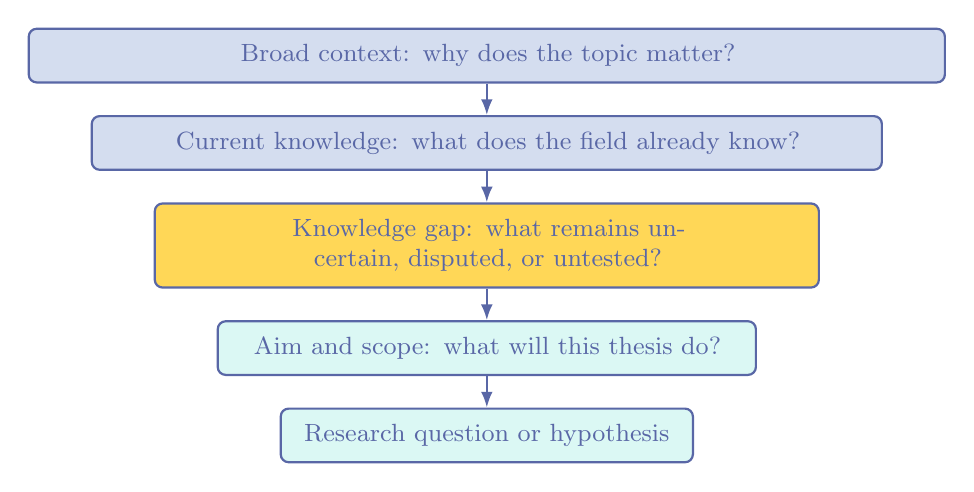
\begin{tikzpicture}[
    every node/.style={
      draw=GuideBlueDark,
      rounded corners=1mm,
      align=center,
      inner ysep=2mm,
      font=\small
    },
    every path/.style={GuideBlueDark,thick}
  ]
    \node[fill=GuideBlue,text width=11.4cm] (context) at (0,0)
      {Broad context: why does the topic matter?};
    \node[fill=GuideBlue,text width=9.8cm,below=4mm of context] (field)
      {Current knowledge: what does the field already know?};
    \node[fill=GuideGold,text width=8.2cm,below=4mm of field] (gap)
      {Knowledge gap: what remains uncertain, disputed, or untested?};
    \node[fill=GuideGreen,text width=6.6cm,below=4mm of gap] (aim)
      {Aim and scope: what will this thesis do?};
    \node[fill=GuideGreen,text width=5.0cm,below=4mm of aim] (rq)
      {Research question or hypothesis};
    \draw[-{Latex[length=2mm]}] (context) -- (field);
    \draw[-{Latex[length=2mm]}] (field) -- (gap);
    \draw[-{Latex[length=2mm]}] (gap) -- (aim);
    \draw[-{Latex[length=2mm]}] (aim) -- (rq);
  \end{tikzpicture}
  \caption[The introduction funnel]{The introduction funnel. The focus narrows from the broader scientific context to the research question. Each level should make the next one feel necessary, rather than lowered from the ceiling  by an unseen crane.}
  \label{fig:funnel}
\end{figure}

Figure~\ref{fig:funnel} is a planning device, not a requirement that every introduction contain five paragraphs of identical length.
Some theses need more context; others need a longer explanation of the gap.
The direction, however, should remain visible throughout.

Now, there are also wrong ways to do this, such as the following example:
\begin{avoidbox}{A funnel that is more like a bowl}
Climate change is a big problem. Renewable energy is very important. Wind power is used in many countries. This thesis investigates wind power.
\end{avoidbox}
I mean, this is a bit too on-the-nose, but the idea is simple.
Note that the claims here are maybe all true -- but they are a value judgement that is not motivated.
To state something is a `big problem' neither explains why it is a problem nor the impact it has.
Moreover, `big' is relational to something else.
It really begs the question, `big compared to what?' Likewise, `very important' is a value judgement that is not motivated.
Try to stay clear from this language -- although this is the way we speak in everyday life, it is not the way we write a thesis\footnote{If this document is still around in 50 years, go look back at the crazy president the United States of America had in 2026. Donald Trump. He spoke just like this. But he was much more on the line that climate change was a hoax...}.
Unless, maybe, if your thesis is about rapping, hip hop, or generally about being a cool human being.


\begin{betterbox}{A funnel that arrives somewhere}
Climate change can severely impact the availability energy resources around the globe.
Extreme events, such as heat waves, droughts, and floods, are expected to become more frequent and intense as the climate warms.
Wind dynamics are known to be affected by global warming, which may change the frequency and magnitude of wind-power ramps.
Short wind-power ramps influence balancing requirements, yet the impact of the change of their frequency on the existing and future power system is not well understood.\footnote{I should add a note here that 1) this moves too quickly, 2) you will need to include citations to support your claims, which I am not doing here, since this is just an example, and 3) this is just the start of the funnel -- you have to arrive at the research question, which is not done yet.}
\end{betterbox}

The stronger version identifies a phenomenon, its possible consequences, a specific operation, and starts narrowing the question to what a topic of a thesis might be.
This should lead in a natural way to a research question.

\subsection{Ask a research question that can be answered}

A research question should be clear, bounded, and answerable using the available data, methods, time, and ethical permissions.
`How can renewable energy save the world?'\footnote{I mean, if you can answer this question in your master thesis, please give me a call, I would love to read it. Truly.} is ambitious, but it is not a Master's project.
`How does temporal aggregation affect estimated wind-power ramp rates?' is a good start, as it can be connected to a method and an observable result.
You will likely have to be more detailed than this, because even this research question lacks sufficient depth.

Depending on the discipline, the central question may be accompanied by subquestions, hypotheses, or objectives.
These devices are useful only when they divide the same problem.
Five unrelated questions do not form a more impressive thesis; they form a small research programme with one exhausted student\footnote{Yup, that is you, thinking about that pottery class you once took and wondering if life as a baker might have been easier.}.
Three sub-questions are usually enough.
There is no correct number, but more is not better.

\begin{thesispoint}{A useful test for every research question}
Can the question be answered in the conclusion using evidence presented in the results and interpreted in the discussion? If the honest answer is `ahhhh, well, like, maybe?', the question or the project scope should change.
\end{thesispoint}

The introduction normally ends with a short roadmap.
One paragraph is usually enough: state what each major section contributes to the argument.
Avoid a tourist itinerary such as `Section 2 contains theory, Section 3 contains methods, Section 4 contains results, Section 5 is my collection of cat pictures from the internet, Section 6 discusses the findings in this thesis, and Section 7 closes with some final remarks' (maybe skip Section 5)\footnote{We have not discussed much about \LaTeX but each section \texttt{\textbackslash section} should have a label \texttt{\textbackslash label}, which you can use to refer to with \texttt{\textbackslash ref}.}.

\subsection{Use an academic voice, not an academic fog machine}

Academic writing should be precise, calm, and appropriately cautious -- think, grandfather's voice.
It need not sound as though every sentence was issued by a committee in 1789\footnote{The good old times of the French revolution, where every aristocrat had an idea how someone else should lead their lives, just not themselves.}.
Prefer ordinary words when they express the meaning accurately.
`Use' is usually better than `utilise'; `because' is often better than `owing to the fact that'.
`Whassup' is not better than `what is happening', but it is also not appropriate in a thesis.

Avoid contractions in the thesis: write `do not', `cannot', `is not', and `we have' rather than `don't', `can't', `isn't' (definitely do not write `ain't'), and `we've'.
Use either the passive voice when the actor is genuinely unimportant, or `we'\footnote{Ahh, now here comes an interesting division. Why would one write `we' in a thesis? Most of the times, a thesis is authored by a single person -- yup, you. It is common to write `we did X' as if you are including the reader as part of the text, so you two together can come to a thesis at the end. This is not a must, but it is generally a nice way to write.} when the researchers made a decision that should remain visible.
Be consistent, and consult the supervisor if the discipline follows a different convention\footnote{Some disciplines in Mathematics and Geology prefer to write theses in French. Mon oeil, c'est du pipeau!}.


\begin{table}[ht]
  \centering
  \small
  \caption[Examples of clearer academic sentences]{Examples of weak and more
  precise academic sentences. The appropriate wording depends on the evidence and the research design.}
  \label{tab:academic-voice}
  \begin{tabularx}{\textwidth}{@{}p{0.18\textwidth}YY@{}}
    \toprule
    Issue & Avoid & Prefer \\
    \midrule
    Contraction
      & The model can't reproduce the peaks.
      & The model cannot reproduce the observed peaks. \\
    \addlinespace
    Hidden decision
      & It was decided that missing values should be removed.
      & We removed observations for which the input data were missing. \\
    \addlinespace
    Vague reference
      & This shows that it is better.
      & The lower root-mean-square error indicates that Model B reproduced the observations more accurately. \\
    \addlinespace
    Causality
      & Wind generation caused the price decrease.
      & Higher wind generation was associated with lower day-ahead prices during the study period. \\
    \bottomrule
  \end{tabularx}
\end{table}

Now, a few rules are important.
Not too many, but a few.
Table~\ref{tab:academic-voice} shows several common repairs that improve academic writing.
I would like to particularly advise you against the `hidden decision' issue, as it is very common in theses.
Note that a theses is \emph{not a report} of the way you did your work.
It is a report on the methods and results of your work, with justification and discussion.
What does this mean? It means that you should not write things like `I decided to do this, and then I did that, and then I did this other thing.'
State instead what is relevant to the decisions: `Due to the limited data in 2022, we used a data augmentation technique to increase the number of training samples for the model.' (note how you never have to write `I decided X', you just state the reason for your choices.)

Paragraphs also need structure.
By the end of your thesis, your dorm room will also need structure, but that is a different story.
A useful scientific paragraph begins with one claim or topic, develops it with evidence or reasoning, and ends by explaining its relevance or creating a transition.
A paragraph is not a storage cupboard for sentences that happened to concern approximately the same noun.
This is a general rule, there are also less useful paragraphs here and there, and that is fine.

\clearpage
\section{Theory: build only what you need}\label{sec:theory}

The theory section gives the reader the concepts, models, and notation needed to understand the research question, methodology, and results.
It is not a small encyclopaedia written to demonstrate that many textbooks were available and how smart you are.
Although you might be very smart.
Very very smart.
Who really knows?

Now, most of the times when you get to the theory section, you might have a feeling that you will have to `plagiarise' a lot of text from a book or a paper.
Well, how do I put this nicely\dots you can use books or papers quite closely for your theory, and yes, generally speaking, this will feel very close to the part of your thesis that is just `copy-paste' from a book or a paper, but you should not copy the text as is.
This is not strange.
No one is here to reinvent Newton's laws of motion, or the Navier-Stokes equations, or the laws of thermodynamics.
Actually, a very good way to start a theory section is to states explicitly `this section follows closely the book (insert book title) by X and Y'.
This is a very good way to start, as it gives credit to the authors of the book.
Just avoid the `Ctrl-C' and `Ctrl-V' approach, as this is not a good way to write a thesis\footnote{Yes yes, all of you MAC aficionados, use your Apples to copy and paste\dots apples apples.} (plus, plagiarism is treated very seriously by any university. Do not plagiarise!)

\begin{thesispoint}{What the theory section must accomplish}
Define the central concepts, state the assumptions behind the models, introduce the notation, and establish the relationships that will be used later. 
Include what the reader needs to follow the argument; omit material that never returns.
If it is boring, you are doing a good job.
If it is very boring, throw in a joke or two for good measure.
\end{thesispoint}

Now, theory comes with equations\footnote{Equations are close to the most beautiful things one can find in the world. Just wanted to say that.} some of the time.
Equations are sentences in another notation.
Mathematics is just another language.
It is a quite helpful language, except I would not generally advise it for dating, it can lead to some confusion.
Equations\footnote{not formulas, do not use the word `formulas' in a thesis, it is just not as elegant as equations\dots It is actually inadequate, generally speaking -- and uncool if you want to have mathematicians as friends, which, duh, you obviously do!} are part of the argument, and they must be treated as such.
They should be introduced, punctuated, numbered when they are referenced, and followed by definitions.

For example, the kinetic power passing through the swept area of a wind turbine is given by
%
\begin{equation}
P_\mathrm{wind} = \frac{1}{2}\rho A v^{3}, \label{eq:wind-power}
\end{equation}
%
where \(P_\mathrm{wind}\) is the power in \unit{W}, \(\rho\) is the air density in \unit{kg\,m^{-3}}, \(A\) is the swept area in \unit{m^{2}}, and \(v\) is the wind speed in \unit{m\,s^{-1}}.\footnote{If you are not too familiar with \LaTeX, the \texttt{\textbackslash label} command is used to label the equation, and the \texttt{\textbackslash eqref} command is used to refer to it later.}

Now, things to notice here: Always introduce the terms in the equation, in this case, \(P_\mathrm{wind}\), \(\rho\), \(A\), and \(v\).
You do not need to do this again in the next equation, so if the next equations used the same symbols, you do not need to introduce them again -- but of course you have to introduce any new symbols you use in the next equations.
Now, when referring to the equation, always use the equation number, in this case, \eqref{eq:wind-power} (\verb|\eqref{eq:wind-power}|, where \verb|\eqref| is generally preferred over \verb|\ref|, as it includes the parenthesis).
It is your choice to use the word `Equation', `Eq.', or nothing and just refer to the number, when referring to an equation, but be consistent throughout the thesis\footnote{If you want to really annoy scientist, you should just be inconsistent. I caution you against this as we are known hold grudges for centuries.}.

When possible, include the units of the symbols, as this is very helpful for the reader.
It is also a good point to mention if another scale is more convenient, such as using \unit{MW} instead of \unit{W}, or \unit{km\,h^{-1}} instead of \unit{m\,s^{-1}}.

\begin{avoidbox}{Equation by ambush}
Dropping an unexplained formula into the text, changing symbols three pages
later, and hoping that the reader recognises the model from undergraduate
lectures will lead you to anger the ancient gods of Mathematics and Leibniz will haunt your dreams for \(e^{42}\) seconds.
\end{avoidbox}

\begin{betterbox}{Equation with a job}
Introduce why the relationship is needed, define every symbol at first use,
state the assumptions and valid range, cite the source, and explain how the
equation will be used in the analysis.
\end{betterbox}


Use notation consistently\footnote{I always like the Norwegian term for this: `konsekvent' (the direct root translation in English leads to `consequent', but the norwegian relates more with consistency).}.
A symbol should not denote wind speed in Section~\ref{sec:theory} and voltage in the results unless the change is both necessary and unmistakable.
A symbol should also not refer to two different quantities.
Units should follow the SI system, values should carry sensible precision\footnote{You just have to think back to your time in FYS101 or FYS102 learning about significant figures or `gjeldende sifre'. If you do not remember how this works, the university will install a new brain in your head.}, and every logarithm should make clear what enters it.
The reader should not need to infer whether ``10'' means \qty{10}{s},
\qty{10}{MW}, or ten unusually cooperative wind turbines.

\clearpage
\section{Literature Review: Synthesis, or another complicated word for `summary'}
\label{sec:literature}

The literature review explains how the thesis sits within existing knowledge.
Its purpose is not to prove that many PDFs were downloaded\footnote{Some from very shady websites on the internet\dots but your supervisor does not need to know that.}.
It should identify what is known, where findings agree or conflict, how methods differ, and what gap motivates the present study.
Detective work, really.

But hold on, some of you might be wondering `my supervisor did not tell me to write a literature review, so I do not have to do it, right?'
Here is a somewhat of a difference between a Master's of Science thesis and Sivilingeer thesis in Norway\footnote{This is equivalent to most Engineers' `Final Project', which we conflate to a thesis, as they close a Master's degree}.
There is some freedom here, since this is not a strict requirement for theses, but I know what you are thinking: `So\dots I do not have to read all those boring academic papers?'
\dots
I think you know the answer, right?



\begin{thesispoint}{What the literature review must accomplish}
Organise the literature around concepts, methods, debates, or findings that matter to the research question.
Compare studies and end each part by stating what the comparison means for this thesis.
I always like to think about this as, `what is up in Science at the moment, and where does my thesis fit in?'
\end{thesispoint}

\begin{avoidbox}{The author-by-author parade}
Author A studied wind ramps and found X. Author B studied wind ramps and found Y.
Author C studied wind ramps and found Z. Author D also owned a computer.
\end{avoidbox}

Now, a literature review is not a list of papers.
The idea is to build a narrative that explains what is known in the relevant Science of your field.
The best approach to start with is to take one of the scientific publications and try to write a two-paragraph summary of it.
It is important to find a good structure to make these summaries.
Present the paper\footnote{In Science, we often called \emph{scientific articles} simply \emph{papers}.} by introduce what is the target of the authors.
Try to explain, in some sense, what is the research question of the paper.
Then, explain the methods used to answer the research question.
Note that sometimes, the methodologies can be quite complicated.
Try to explain it the best you can.
Then, explain the results of the paper, and finally, explain the interpretation of the results.

Now, multiply this by ten. Fifteen is better. Yup\dots lots of work. Jolly good fun.


\begin{betterbox}{A synthesis}
Studies using minute-resolution observations report heavier ramp-rate tails than studies based on hourly averages.
The estimates are therefore not directly comparable: temporal aggregation suppresses short fluctuations, while the choice of normalisation changes the apparent scale. These methodological differences motivate the resolution sensitivity test used in this thesis.
\end{betterbox}

The stronger paragraph compares findings, identifies a reason for the
difference, and links that comparison to the methodology. A synthesis may still
name individual authors, particularly when their interpretation matters, but
the paragraph should be organised by an idea rather than by the order in which
papers were opened.

Citations should be placed close to the claims they support. Several sources
may be cited together with
\verb|\parencite{Booth2016craft,Swales2012academic}|, which produces the combined
citation~\parencite{Booth2016craft,Swales2012academic}. When an author is part of
the sentence, use \verb|\textcite{Booth2016craft}|; for a particular passage,
add a page number with \verb|\parencite[p.~32]{Booth2016craft}|.

Prefer primary sources for original findings and methods.
Reviews are useful for orientation and synthesis, but citing a review does not establish that the original article was read.
Reports, datasets, software, standards, theses, and web sources also require complete references.
A URL\footnote{That is a link for you boomers out there!} on its own is not a bibliography entry, and `Google' is not the author of everything found through a search engine.
Advisable to find cooking recipes, but generally just citing Google is not a good idea for a thesis.
Unless they are paying you very well, and then you should probably consider a career change.
`Grandma' is also not a valid source, even if she is very wise and has four PhDs on the topic.

\begin{latexnote}{Bibliography habits that prevent later misery}
Store each source in \texttt{bib.bib} when it is first used. Include a DOI when
one exists, retain the stable URL and access date for web sources, and use the
correct entry type. Use \texttt{@article} for journal articles,
\texttt{@inproceedings} for conference proceedings, and \texttt{@thesis} for
Master's and PhD theses. For a thesis, include the institution, year, and a
repository URL when available.
\end{latexnote}

Paraphrasing changes more than a few words. Read the source, put it aside,
explain the idea in the logic of the present argument, compare the result with
the original, and cite it. A citation does not make copied syntax or borrowed
reasoning automatically acceptable. Likewise, any use of generative tools must
follow the current programme rules; responsibility for every statement,
calculation, and reference remains with the author.

\clearpage
\section{Methodology: Leave a Reproducible Trail}
\label{sec:methods}

The methodology explains what was done and why the chosen approach can answer the research question.
Now, most of the times, it is actually difficult to distinguish the theory and the methodology, as they are very closely related.
Think about it in this way: Theory is the mathematics and models that you are using; Methodology is the way you are using them, and how you are applying them to your data (so here all the details, parameters, numbers, etc., matter!)

One very important thing: The methodology should be detailed enough for another trained researcher to repeat the work, assess the choices, and understand the sources of uncertainty.
It should not recreate Tuesday afternoon in chronological order.
Although Tuesdays are generally very nice days.

\begin{thesispoint}{What the methodology must accomplish}
Identify the data or materials, describe collection and processing, justify the analysis, state assumptions and exclusions, quantify uncertainty, address ethical considerations, and explain how the work can be checked or reproduced.
\end{thesispoint}

A useful methodology answers the following questions in a logical order:

\begin{enumerate}
  \item What data, samples, instruments, participants, or models were used, and
  where did they come from?
  \item How were they selected, calibrated, cleaned, transformed, or excluded?
  \item Which parameters, thresholds, boundary conditions, and software
  versions were used?
  \item Which statistical or numerical methods were applied, and why were they appropriate?
  \item How were uncertainty, sensitivity, bias, missing data, and possible
  failure modes assessed?
  \item Which ethical approvals, licences, or data restrictions apply, and
  where can permitted data and code be found?
\end{enumerate}

\noindent (Note that not all the point will apply to your thesis.)
A small remark: You do not need to state that you have used Python 3.14.2 with the package \texttt{NumPy} version 1.25.0, unless it is relevant to the results.
Generally, you can reserve a very small paragraph for the software and packages you have used (and their versions, only if that is actually important).

\begin{avoidbox}{A laboratory diary}
First, I downloaded the file.
Then I opened Python.
Then there was an error, so I had lunch.
Afterwards, I tried another file and it worked.
I realised that if I pressed the big green button twice, the plot would appear.
Then I spent 10 minutes trying to understand why there where peanuts on the bottom of my backpack.
\end{avoidbox}

\begin{betterbox}{A reproducible procedure}
We downloaded hourly observations for 2020--2025 from the SuperDuperCool repository.
Duplicate timestamps were removed, missing intervals were
retained as missing, and series with less than \qty{95}{\percent} completeness were excluded.
\end{betterbox}

The passive voice is useful when the procedure matters more than the actor:
`The sensor was calibrated before each run.'
Use `we' when agency clarifies a scientific decision: `We selected the threshold before inspecting the group differences.'
Avoid the first-person singular unless the discipline or supervisor explicitly prefers it.
Past tense usually describes what was done;
present tense is normally used for established relationships, definitions, and what a figure shows.
So, I generally think it is better for the theory, literature, and methodology, since they represent past work and past choices.
The presentation of the results and discussion is a bit more flexible, as they represent your own work and your own interpretation of the results.
It makes more sense to write `Figure X shows' than `Figure X showed' in the results.
In the discussion, this is a bit of a mix.
You can both refer to the figures in the past or in the present, but your discussion takes place in the present.

One important thing to consider is what to do with, let us call them, \emph{less good} results?
At some point, you might be wondering, `should I include this result in my thesis?'
Is it good?
Is it good enough?
Well, here we need a distinction: Results can be less good because the methodology for a particular part of the work was not adequate.
Imagine running an experiment and realising that part of your results are muddle because you have used only half of the total solvent that you should have.
This is a methodological issue, and unless there is still something clearly interesting to be learned from the result, it is probably better to exclude it from the thesis.
On the other hand, results can be less good because they are not what you expected, because your mathematical model can only capture a portion of the phenomena or the data is scarce.
I would advise you to include these results.
Note that progress in science is often made by negative results.
Maybe your Super-Duper Machine Learning Model 1000 Max proves worse than the local tarot card reader in town.
Well, that is a result in itself, that the Super-Duper Machine Learning Model 1000 Max is generally a weak model for the problem.
That is a result in itself -- maybe not the one you wanted, but oh well, now it is midnight and you have to go to bed.

\clearpage
\section{Results: Let the Evidence Do Some Work}\label{sec:results}

The results section presents the evidence needed to answer the research
questions. Organise it by question, hypothesis, or analytical step rather than
by the dates on which plots were produced. Begin each subsection with the
result being examined, present the evidence, quantify uncertainty, and state the
immediate observation. Save the broader meaning for the discussion.

\begin{thesispoint}{What the results section must accomplish}
Present relevant findings clearly, report uncertainty and sample sizes, direct
the reader to every table and figure, and distinguish observations from later
interpretation. A result that never contributes to a research question may
belong in an appendix, a repository, or the fond memories of the author.
\end{thesispoint}

Figure~\ref{fig:side-by-side} illustrates a two-panel figure intended to occupy
the full text width. It is introduced before it appears and is referenced by
number. Scientific writing should not refer to ``the figure below'' or ``the
table above'', because floats may move and readers deserve coordinates more
reliable than weather forecasts.

\begin{figure}[!b]
  \centering
  \includegraphics[width=\textwidth]{side-by-side.pdf}
  \caption[Example of a full-width two-panel figure]{Example of a full-width
  two-panel figure. Related panels are placed side by side to support direct
  comparison. Axis labels, units, tick labels, and legends must remain legible
  at final print size; if the reader has to zoom to \qty{300}{\percent}, the
  figure has become an eyesight test. The full caption should define the panels,
  lines, symbols, and uncertainty displays, and should state the main message
  without requiring a search through the body text.}
  \label{fig:side-by-side}
\end{figure}

Every figure and table needs a numbered caption and a label. Use a short caption
for the lists at the front and a self-contained full caption in the document.
The three relevant lines may look as follows:

\begin{quote}
\ttfamily
\textbackslash caption[Short caption]\{Full caption\}\\
\textbackslash label\{fig:wind-ramp-pdf\}\\
Figure\textasciitilde\textbackslash ref\{fig:wind-ramp-pdf\}
\end{quote}

Place the label immediately after the caption. The tilde prevents an
unfortunate line break between the word and its number.

Choose a representation that serves the comparison. Use tables when exact
values matter and figures when patterns matter. Avoid decorative three-
dimensional charts, rainbow colour maps, screenshots of plotting windows, and
legends that require colour vision as an entrance examination. Colour choices
can alter the apparent structure of scientific data, so perceptually uniform
and colour-vision-accessible maps should be preferred~\parencite{Crameri2020misuse}.

Do not report more digits than the data support. For example,
\qty{12.438762}{MW} is not necessarily more informative than
\qty{12.4}{MW}; it may merely reveal that the computer owns several decimal
places. State variability, confidence or credible intervals, uncertainty, and
sample size as appropriate. Do not use ``significant'' to mean ``large'',
``interesting'', or ``the supervisor nodded''. If statistical significance is
meant, name the test, statistic, effect size, and threshold.

\clearpage
\section{Discussion: Explain Without Overclaiming}
\label{sec:discussion}

The results tell the reader what was observed. The discussion explains what
those observations mean, how they answer the research question, how they relate
to prior work, which explanations remain plausible, and where the conclusions
stop being secure.

\begin{thesispoint}{What the discussion must accomplish}
Answer the research questions, interpret the most important findings, compare
them with the literature, examine alternative explanations, discuss strengths
and limitations, and state the scientific or practical implications.
\end{thesispoint}

A strong discussion commonly moves through five tasks. First, state the answer
to the relevant research question. Second, identify the result that supports
that answer. Third, compare it with expectations and earlier studies. Fourth,
explain plausible mechanisms and alternatives. Fifth, define the limitations
and implications. The order may change, but none of the tasks should be replaced
by a second tour through every number in the results section.

\begin{avoidbox}{A claim larger than the study}
These results prove that temporal aggregation always causes grid operators to
underestimate balancing requirements.
\end{avoidbox}

\begin{betterbox}{A claim fitted to the evidence}
Within the Norwegian data and resolutions examined here, temporal aggregation
reduced the estimated frequency of large ramp events. This result indicates
that balancing studies based only on hourly data may underrepresent short-term
variability; its effect on operational reserve procurement requires a separate
system-level analysis.
\end{betterbox}

The stronger claim states the scope, the observation, the supported inference,
and the boundary beyond which more work is required. Verbs such as ``shows'',
``indicates'', ``supports'', ``is consistent with'', and ``suggests'' are not
interchangeable decorations. Choose the one that matches the design and the
strength of evidence.

Limitations are not a ritual confession placed one paragraph before the
conclusion. They describe the conditions under which the answer should be
trusted. Explain the likely direction and magnitude of important limitations
where possible. A geographically narrow dataset, a short observation period,
measurement error, modelling assumptions, or non-random missing data may each
change what can be inferred. State what was done to test robustness and what
remains unresolved.

Do not introduce new analyses in the discussion. Evidence supporting an
interpretation belongs in the results. Return useful new ideas to the relevant
section; the thesis is allowed to be revised.

\clearpage
\section{Conclusion: Land the plane, or at least open the parachute}
\label{sec:conclusion}

The conclusion gives a direct and proportionate answer to the problem posed in
Section~\ref{sec:introduction}. It is not a summary of the table of contents,
and it is not the location for a final surprise dataset.

\begin{thesispoint}{What the conclusion must accomplish}
Restate the aim briefly, answer each research question, identify the main
contribution, state the principal limitations or scope, and give specific
recommendations or future work when justified. Introduce no new evidence.
\end{thesispoint}

The conclusion should be understandable without reopening every preceding
section, but it must remain traceable to the evidence already presented. A useful
test is to place the research question and the proposed answer side by side. If
the wording of the answer changes the question, the thesis may have answered a
different problem.

\begin{avoidbox}{The ceremonial conclusion}
In conclusion, this thesis studied a very important topic. Many interesting
results were found. More research is needed in the future.
\end{avoidbox}

\begin{betterbox}{A conclusion with content}
Aggregation from \qty{1}{min} to \qty{15}{min} reduced the estimated frequency
of extreme wind-power ramps in all analysed bidding zones. The effect was
largest in the zones with the highest short-term variability. The result answers
the research question for the 2020--2025 dataset, but does not by itself quantify
changes in reserve procurement. Future work should therefore propagate the
resolution-dependent ramp distributions through an operational balancing model.
\end{betterbox}

Write the abstract after the conclusion. The abstract is a compact account of
the context, gap, aim, method, principal quantitative results, and conclusion.
It is not an invitation to the thesis, a list of chapter titles, or a trailer
that hides the ending. The title should also be checked last: it should be
specific, searchable, accurate, and considerably shorter than the thesis.

The final principle is simple. A reader should never have to guess why a section,
paragraph, figure, equation, or citation is present. Make the research question
visible, build the argument around it, and revise until the shortest defensible
path through the work is also the clearest one. Then make a backup.

% References come before the appendices.
\clearpage
\references

\clearpage
\appendices

\section{The Five-Minute Pre-Submission Audit}
\label{app:audit}

Five minutes is not enough to repair a thesis, but it is enough to discover that
the title still says ``Insert Thesis Title''. Perform this audit earlier than
five minutes before the deadline.

\begin{enumerate}
  \item The title, author, year, credits, faculty, programme, supervisor, and PDF
  metadata are correct.
  \item The abstract states the method, principal quantitative findings, and
  conclusion; it does not promise results that never arrive.
  \item Every research question is explicit and is answered in the conclusion.
  \item Every major claim is supported by evidence, reasoning, or an appropriate
  citation placed close to the claim.
  \item Every symbol, acronym, dataset, method, and software tool is defined at
  first use.
  \item Every figure and table is mentioned in the text, legible at print size,
  numbered, labelled, and supplied with a self-contained caption.
  \item Units, notation, significant figures, spelling, voice, and tense are
  consistent.
  \item Limitations are specific and connected to what can and cannot be
  concluded.
  \item The source compiles without undefined citations, ``??'' references,
  missing files, or important warnings.
  \item Placeholder text, tracked comments, private notes, and the paragraph
  written at \qty{03}{h} ``to fix tomorrow'' have been resolved.
  \item The final PDF has been inspected page by page, not merely trusted because
  LaTeX produced it without visible flames.
  \item The project and data are backed up in a documented location.
\end{enumerate}

\section{Small LaTeX Habits with Large Benefits}
\label{app:latex}

Use labels and references rather than typing numbers manually. For example:

\begin{quote}
\ttfamily
Figure\textasciitilde\textbackslash ref\{fig:side-by-side\}\\
Equation\textasciitilde\textbackslash eqref\{eq:wind-power\}\\
Section\textasciitilde\textbackslash ref\{sec:methods\}
\end{quote}

Use descriptive labels; six months from now, \verb|fig:wind-ramp-pdf| will be
more helpful than \verb|fig:7|.

Write ranges with an en dash in LaTeX source, for example \verb|2020--2025|.
Use \verb|\emph{...}| for emphasis rather than underlining. Keep values and
units together with \texttt{siunitx}, for example
\verb|\qty{12.4}{MW}| and \verb|\unit{m\,s^{-1}}|. Do not insert manual spaces,
page numbers, or section numbers to repair the layout; repair the structure or
the source instead.

Compile the final document with XeLaTeX. In Overleaf, open \emph{Menu}, find
\emph{Compiler}, and select \emph{XeLaTeX}. This gives the intended fonts and
usually produces a compact PDF. Every saved kilobyte makes an exceptionally
small contribution to reducing storage-related emissions, but science is built
from cumulative effects.

Most importantly, compile regularly. Twenty lines of new text produce a useful
error message. Two hundred uncompiled lines produce an escape room.

\end{document}